% Options for packages loaded elsewhere
\PassOptionsToPackage{unicode}{hyperref}
\PassOptionsToPackage{hyphens}{url}
\PassOptionsToPackage{dvipsnames,svgnames,x11names}{xcolor}
%
\documentclass[
  a4paper,
  DIV=11,
  numbers=noendperiod]{scrartcl}

\usepackage{amsmath,amssymb}
\usepackage{iftex}
\ifPDFTeX
  \usepackage[T1]{fontenc}
  \usepackage[utf8]{inputenc}
  \usepackage{textcomp} % provide euro and other symbols
\else % if luatex or xetex
  \usepackage{unicode-math}
  \defaultfontfeatures{Scale=MatchLowercase}
  \defaultfontfeatures[\rmfamily]{Ligatures=TeX,Scale=1}
\fi
\usepackage{lmodern}
\ifPDFTeX\else  
    % xetex/luatex font selection
\fi
% Use upquote if available, for straight quotes in verbatim environments
\IfFileExists{upquote.sty}{\usepackage{upquote}}{}
\IfFileExists{microtype.sty}{% use microtype if available
  \usepackage[]{microtype}
  \UseMicrotypeSet[protrusion]{basicmath} % disable protrusion for tt fonts
}{}
\makeatletter
\@ifundefined{KOMAClassName}{% if non-KOMA class
  \IfFileExists{parskip.sty}{%
    \usepackage{parskip}
  }{% else
    \setlength{\parindent}{0pt}
    \setlength{\parskip}{6pt plus 2pt minus 1pt}}
}{% if KOMA class
  \KOMAoptions{parskip=half}}
\makeatother
\usepackage{xcolor}
\usepackage[inner=2.5cm,outer=2.5cm,top=3cm,bottom=4cm,headsep=22pt,headheight=11pt,footskip=33pt,ignorehead,ignorefoot,heightrounded]{geometry}
\setlength{\emergencystretch}{3em} % prevent overfull lines
\setcounter{secnumdepth}{5}
% Make \paragraph and \subparagraph free-standing
\makeatletter
\ifx\paragraph\undefined\else
  \let\oldparagraph\paragraph
  \renewcommand{\paragraph}{
    \@ifstar
      \xxxParagraphStar
      \xxxParagraphNoStar
  }
  \newcommand{\xxxParagraphStar}[1]{\oldparagraph*{#1}\mbox{}}
  \newcommand{\xxxParagraphNoStar}[1]{\oldparagraph{#1}\mbox{}}
\fi
\ifx\subparagraph\undefined\else
  \let\oldsubparagraph\subparagraph
  \renewcommand{\subparagraph}{
    \@ifstar
      \xxxSubParagraphStar
      \xxxSubParagraphNoStar
  }
  \newcommand{\xxxSubParagraphStar}[1]{\oldsubparagraph*{#1}\mbox{}}
  \newcommand{\xxxSubParagraphNoStar}[1]{\oldsubparagraph{#1}\mbox{}}
\fi
\makeatother


\providecommand{\tightlist}{%
  \setlength{\itemsep}{0pt}\setlength{\parskip}{0pt}}\usepackage{longtable,booktabs,array}
\usepackage{calc} % for calculating minipage widths
% Correct order of tables after \paragraph or \subparagraph
\usepackage{etoolbox}
\makeatletter
\patchcmd\longtable{\par}{\if@noskipsec\mbox{}\fi\par}{}{}
\makeatother
% Allow footnotes in longtable head/foot
\IfFileExists{footnotehyper.sty}{\usepackage{footnotehyper}}{\usepackage{footnote}}
\makesavenoteenv{longtable}
\usepackage{graphicx}
\makeatletter
\def\maxwidth{\ifdim\Gin@nat@width>\linewidth\linewidth\else\Gin@nat@width\fi}
\def\maxheight{\ifdim\Gin@nat@height>\textheight\textheight\else\Gin@nat@height\fi}
\makeatother
% Scale images if necessary, so that they will not overflow the page
% margins by default, and it is still possible to overwrite the defaults
% using explicit options in \includegraphics[width, height, ...]{}
\setkeys{Gin}{width=\maxwidth,height=\maxheight,keepaspectratio}
% Set default figure placement to htbp
\makeatletter
\def\fps@figure{htbp}
\makeatother
% definitions for citeproc citations
\NewDocumentCommand\citeproctext{}{}
\NewDocumentCommand\citeproc{mm}{%
  \begingroup\def\citeproctext{#2}\cite{#1}\endgroup}
\makeatletter
 % allow citations to break across lines
 \let\@cite@ofmt\@firstofone
 % avoid brackets around text for \cite:
 \def\@biblabel#1{}
 \def\@cite#1#2{{#1\if@tempswa , #2\fi}}
\makeatother
\newlength{\cslhangindent}
\setlength{\cslhangindent}{1.5em}
\newlength{\csllabelwidth}
\setlength{\csllabelwidth}{3em}
\newenvironment{CSLReferences}[2] % #1 hanging-indent, #2 entry-spacing
 {\begin{list}{}{%
  \setlength{\itemindent}{0pt}
  \setlength{\leftmargin}{0pt}
  \setlength{\parsep}{0pt}
  % turn on hanging indent if param 1 is 1
  \ifodd #1
   \setlength{\leftmargin}{\cslhangindent}
   \setlength{\itemindent}{-1\cslhangindent}
  \fi
  % set entry spacing
  \setlength{\itemsep}{#2\baselineskip}}}
 {\end{list}}
\usepackage{calc}
\newcommand{\CSLBlock}[1]{\hfill\break\parbox[t]{\linewidth}{\strut\ignorespaces#1\strut}}
\newcommand{\CSLLeftMargin}[1]{\parbox[t]{\csllabelwidth}{\strut#1\strut}}
\newcommand{\CSLRightInline}[1]{\parbox[t]{\linewidth - \csllabelwidth}{\strut#1\strut}}
\newcommand{\CSLIndent}[1]{\hspace{\cslhangindent}#1}

\KOMAoption{captions}{tableheading}
\makeatletter
\@ifpackageloaded{caption}{}{\usepackage{caption}}
\AtBeginDocument{%
\ifdefined\contentsname
  \renewcommand*\contentsname{Table of contents}
\else
  \newcommand\contentsname{Table of contents}
\fi
\ifdefined\listfigurename
  \renewcommand*\listfigurename{List of Figures}
\else
  \newcommand\listfigurename{List of Figures}
\fi
\ifdefined\listtablename
  \renewcommand*\listtablename{List of Tables}
\else
  \newcommand\listtablename{List of Tables}
\fi
\ifdefined\figurename
  \renewcommand*\figurename{Figure}
\else
  \newcommand\figurename{Figure}
\fi
\ifdefined\tablename
  \renewcommand*\tablename{Table}
\else
  \newcommand\tablename{Table}
\fi
}
\@ifpackageloaded{float}{}{\usepackage{float}}
\floatstyle{ruled}
\@ifundefined{c@chapter}{\newfloat{codelisting}{h}{lop}}{\newfloat{codelisting}{h}{lop}[chapter]}
\floatname{codelisting}{Listing}
\newcommand*\listoflistings{\listof{codelisting}{List of Listings}}
\makeatother
\makeatletter
\makeatother
\makeatletter
\@ifpackageloaded{caption}{}{\usepackage{caption}}
\@ifpackageloaded{subcaption}{}{\usepackage{subcaption}}
\makeatother

\ifLuaTeX
  \usepackage{selnolig}  % disable illegal ligatures
\fi
\usepackage{bookmark}

\IfFileExists{xurl.sty}{\usepackage{xurl}}{} % add URL line breaks if available
\urlstyle{same} % disable monospaced font for URLs
\hypersetup{
  pdftitle={GovCT2},
  pdfauthor={Martin Franke},
  colorlinks=true,
  linkcolor={blue},
  filecolor={Maroon},
  citecolor={Blue},
  urlcolor={Blue},
  pdfcreator={LaTeX via pandoc}}


\title{GovCT2}
\author{Martin Franke}
\date{}

\begin{document}
\maketitle

\renewcommand*\contentsname{Table of contents}
{
\hypersetup{linkcolor=}
\setcounter{tocdepth}{3}
\tableofcontents
}
\listoffigures
\listoftables

\section{Context}\label{context}

In a power plant, a governor regulates the mechanical power (\(P_m\)) or
torque (\(T_m\)) delivered from the turbine to the electrical generator.
This governor model includes the turbine dynamics, i.e.~it takes a
reference power and generator speed and outputs the mechanical torque.

This GovCT2 is a modification of the GovCT1 in order to represent the
frequency-dependent fuel flow limit of a specific gas turbine
manufacturer. Both are based on \emph{Rowen's model} from 1983 {[}1{]}.

When comparing to older standards: GovCT2 is identical to GGOV2 and
GovCT1 is identical to GGOV1.

GovCT2 is part of the CIM/CGMES standard, see {[}2{]} and {[}3{]}. CIM
is developed by ENTSO-E and aims at ensuring the reliability of grid
models and market information exchanges. ENTSO-E developed CGMES as a
superset of the IEC CIM standards (belonging to IEC CIM16) in 2013 to
fulfill the requirements of transmission system operators and their data
exchanges.

The following information has been gathered from {[}2{]}, {[}4{]} and
{[}3{]}.

\section{Model use, assumptions, validity domain and
limitations}\label{model-use-assumptions-validity-domain-and-limitations}

General model for any prime mover with a PID governor.

For example used for:

Can be used to represent a variety of prime movers controlled by PID
governors, such as:

\begin{itemize}
\tightlist
\item
  Single shaft combined cycle turbines and Gas turbines
\item
  Diesel engines (with modern digital or electronic governors)
\item
  Steam turbines with

  \begin{itemize}
  \tightlist
  \item
    steam supplied from a large boiler drum
  \item
    or steam supplied from a large header with approximately constant
    pressure (over the time period of the simulation)
  \end{itemize}
\item
  Simple hydro turbines in dam configurations with

  \begin{itemize}
  \tightlist
  \item
    short water column length
  \item
    and minimal water inertia effects
  \end{itemize}
\end{itemize}

The model is a positive-sequence RMS model, hence it assumes symmetrical
operating conditions and neglects high-frequency dynamics. This type of
model is often used in large-scale stability studies, for which it
reflects the relevant phenomena. It is not a detailed physical model of
the unit. Also for some stability phenomena (e.g.~resonance stability)
this model is not sufficient and EMT models or other approaches may be
necessary.

\section{Model description}\label{model-description}

\subsection{Model schema}\label{model-schema}

\begin{figure}

\centering{

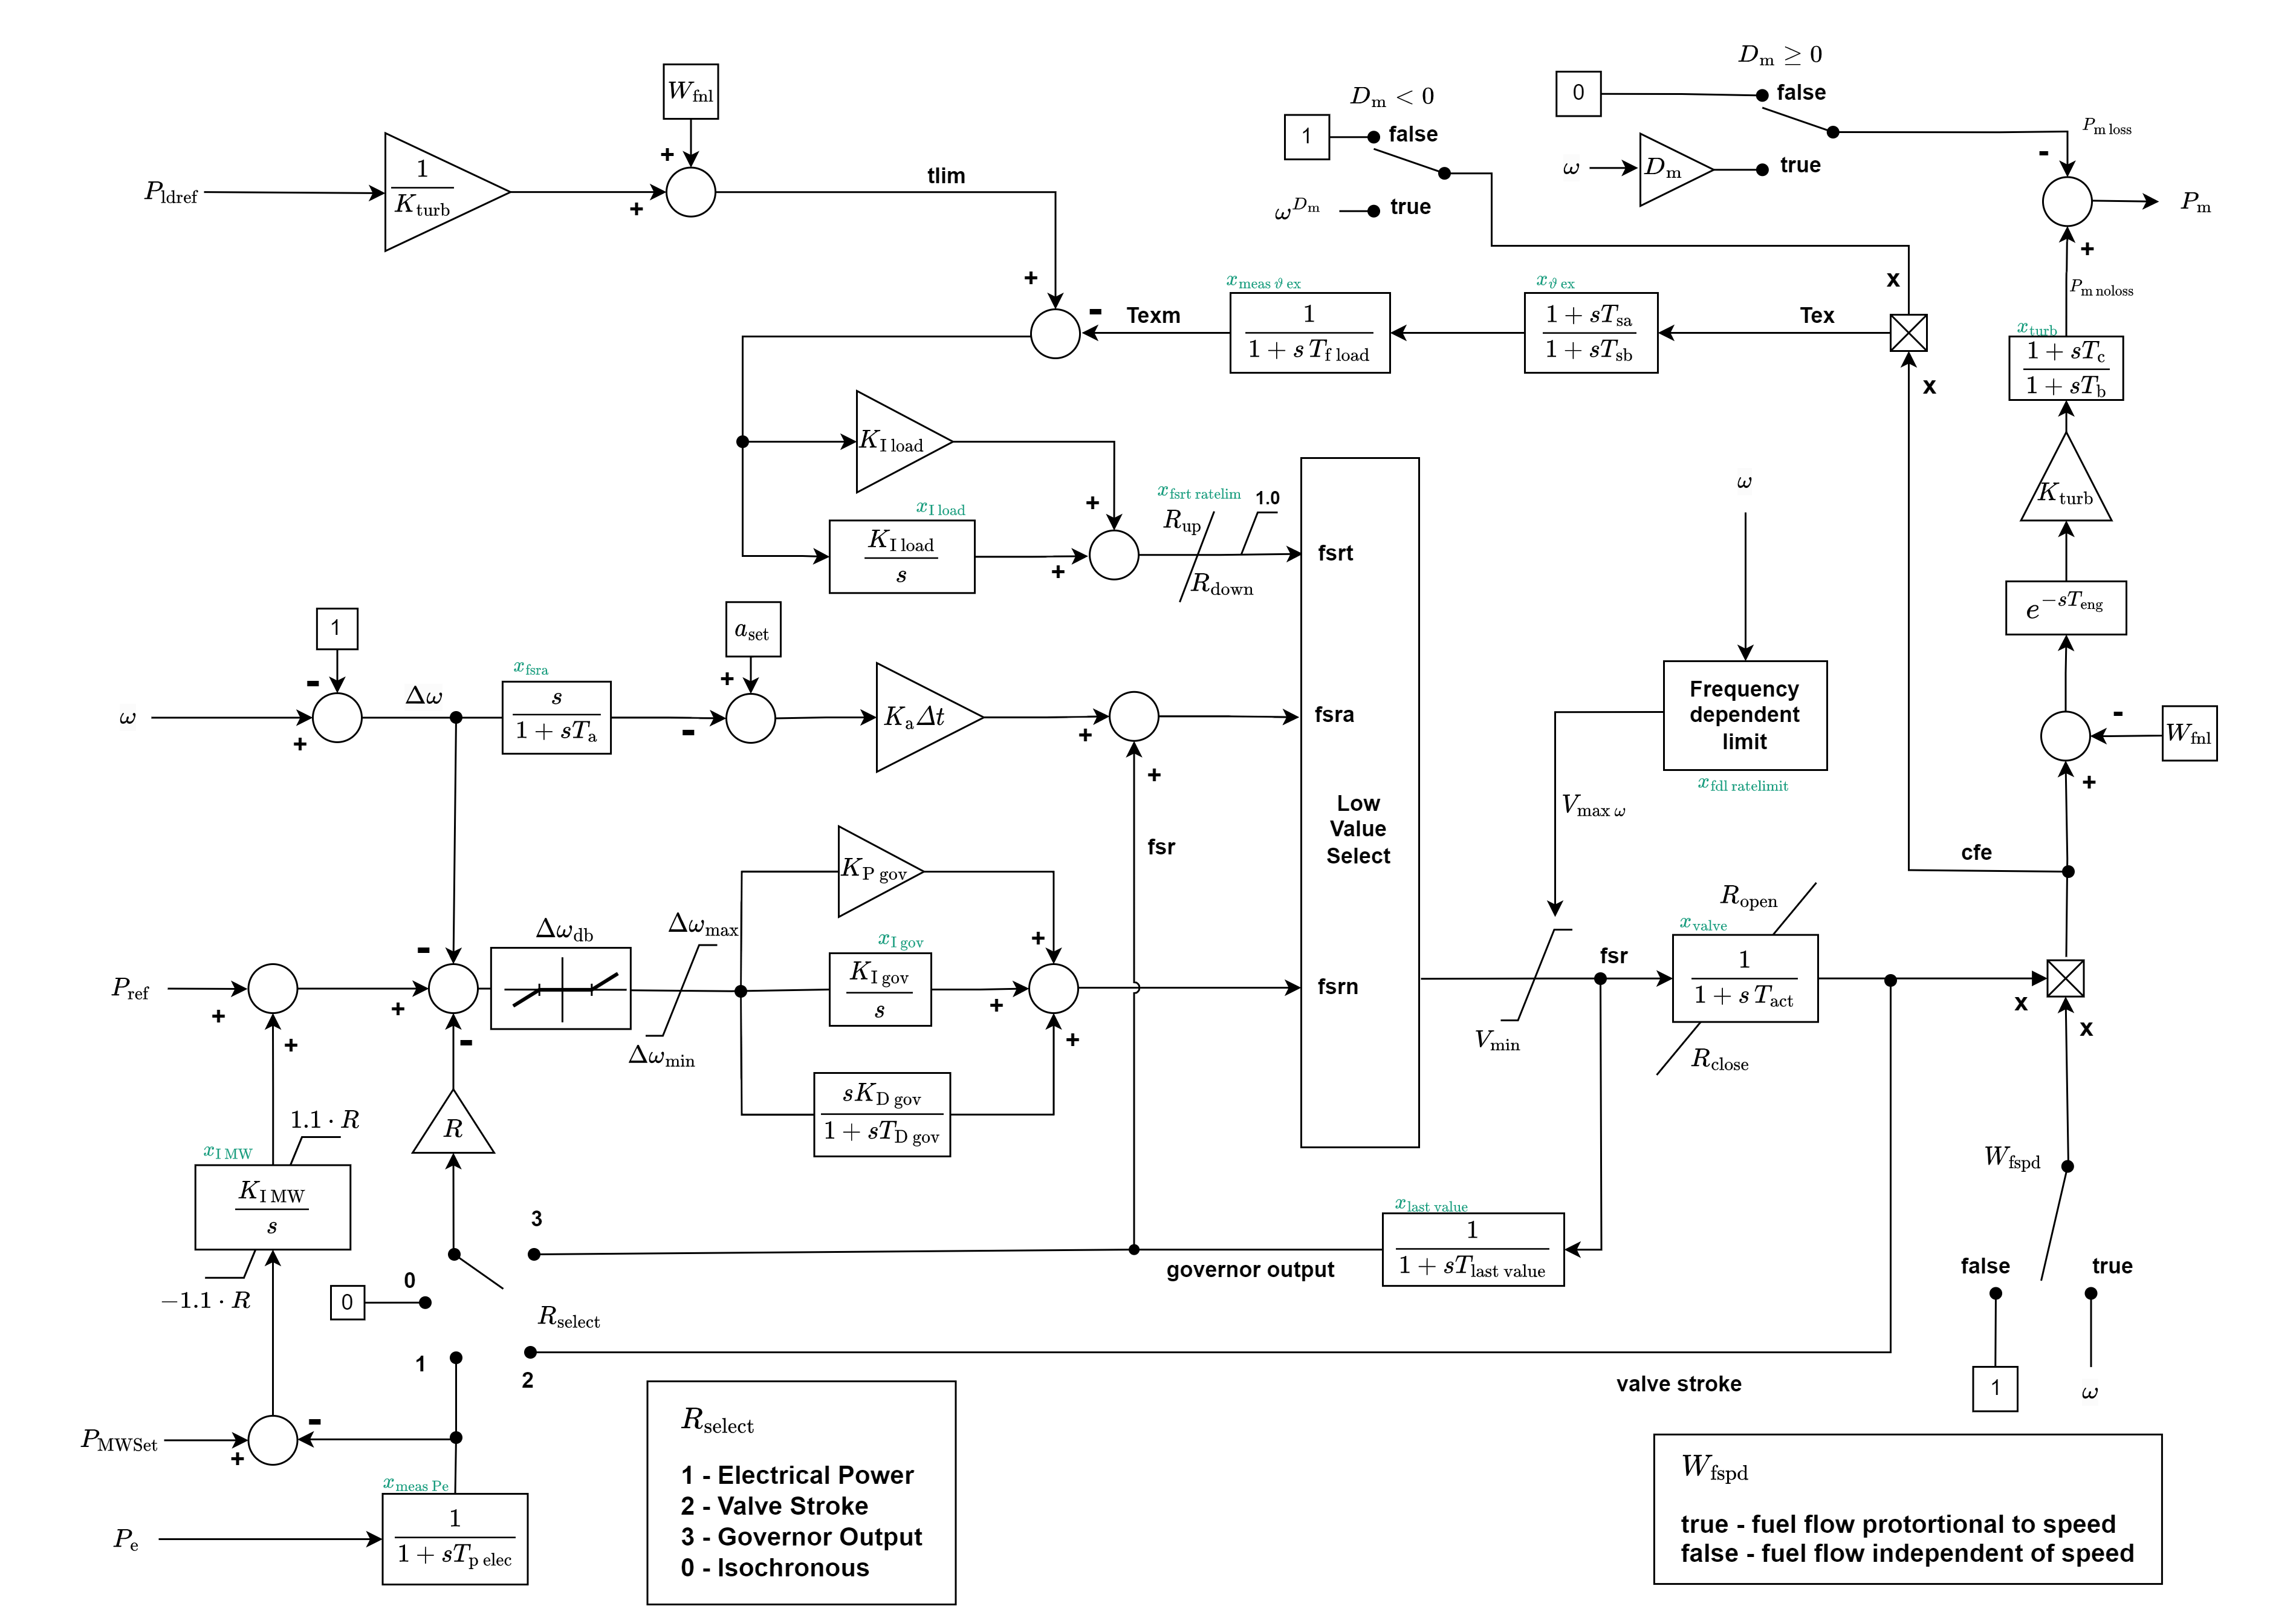
\includegraphics{drawings/GovCT2.drawio.png}

}

\caption{\label{fig-modelSchema}Model schema, based on {[}3{]}}

\end{figure}%

\subsection{Major control paths}\label{major-control-paths}

The following section is based on {[}1{]} (p.~517f).

The model has three major control paths (speed/load, acceleration,
temperature) associated with the dynamic response during disturbances.
Outputs of these control functions are all inputs into a minimum value
selector determining the least fuel request. This is then given to the
actuator.

\subsubsection{Speed/load (fsrn)}\label{speedload-fsrn}

This can be considered the main control path. It corresponds directly to
the governor. The inputs are load demand \(P_\mathrm{ref}\), rotor speed
\(\omega\) and automatic generation control power \(P_\mathrm{MWSet}\).

The resulting signal is then passed through a deadband, limits and a
PID-controller. To represent a specific governor, some elements can be
deactivated by setting parameters to zero (examples in {[}1{]}).

\paragraph{Supervisory load
controller}\label{supervisory-load-controller}

In {[}3{]} the \(P_\mathrm{MWSet}\) path is described as an optional
additional outer loop associated with a power plant control (supervisory
load controller). This is active when \(K_\mathrm{I\,MW}\) is not equal
to zero. It is a slow acting reset control and it adjusts the speed/load
reference of the turbine governor to maintain the electrical power of
the unit at the value which it has been initialized with. That value is
stored in \(P_\mathrm{MW\,set}\) when the model is initialized, and can
be changed during simulation. The load controller is expected to have a
slow reaction compared to the speed governor. {[}3{]}

A value \(K_\mathrm{I\,MW}\) = to 0.01 corresponds to a time constant of
100 s; 0.001 corresponds to 1000 s (relatively slow acting) {[}3{]}.

\paragraph{Acceleration (fsra)}\label{acceleration-fsra}

\begin{quote}
{[}\ldots{]} for studies of large power systems, {[}the acceleration
control loop{]} can be ignored. It is important for islanding studies
and smaller power systems with large frequency variations. If the
generating unit begins to accelerate at a rate over
{[}\(a_\mathrm{set}\){]} (pu/s\^{}2) then this control loop acts to
limit fuel flow. {[}1{]}
\end{quote}

It can be disabled by setting \(a_\mathrm{set}\) to a large value, such
as 1. {[}3{]}

\paragraph{Temperature (fsrt) / load
limit}\label{temperature-fsrt-load-limit}

The load limiter module allows to set a maximum output limit
\(P_\mathrm{ldref}\). This can also model an exhaust temperature limit,
in which case \(P_\mathrm{ldref}\) is not to be interpreted as a power
value. The time constant \(T_\mathrm{f\,load}\) should match the
measurement time constant for temperature (or power or which ever signal
is being modelled). Additionally, the gains of the limiter,
\(K_\mathrm{P\,load}\) and \(K_\mathrm{I\,load}\), should be set to
achieve fast and stable control when the limit \(P_\mathrm{ldref}\) is
reached. To deactivate the load limit, set the parameter
\(P_\mathrm{ldref}\) to a high value {[}3{]}.

The lead-lag block with \(T_\mathrm{sa}\) and \(T_\mathrm{sb}\) can be
used to model the exhaust gas temperature measurement system in gas
turbines. A ``radiation shield'' component of larger gas turbines can be
modeled by setting \(T_\mathrm{sa}=4\,\mathrm{s}\) and
\(T_\mathrm{sb}=5\,\mathrm{s}\), for example {[}3{]}.

\begin{quote}
The temperature limit {[}tlim{]} in pu corresponds to the fuel flow
required for 1 pu turbine power. {[}1{]}
\end{quote}

\subsubsection{Turbine/engine model}\label{turbineengine-model}

The output from the low value select block is given to the first order
lag element representing the fuel or gate system (Valve). {[}1{]}

\(V_\mathrm{max}\) and \(V_\mathrm{min}\) represent the maximum and
minimum fuel valve opening. \(W_\mathrm{fspd}\) is the fuel flow
multiplyer.

\(W_\mathrm{fnl}\) is the fuel required to run the compensator {[}1{]}.

The range of fuel valve travel and of fuel flow is unity, so the limits
lie between 0 pu and 1 pu. \(V_\mathrm{max}\) can be reduced below 1,
for example to model a load limit defined by the operator or supervisory
controller {[}3{]}. Additionally there is a dynamic frequency dependent
limit reduction, see Section~\ref{sec-freqDepLimit}.

For a gas turbine, in the presence of a minimum firing limit,
\(V_\mathrm{min}\) normally is set greater than zero and less than
\(W_\mathrm{fnl}\) {[}3{]}.

The value of the fuel flow at maximum power shall be \(\leq 1\),
depending on the value of \(K_\mathrm{turb}\) {[}3{]}. It translates the
fuel consumption (or water flow) to mechanical power output {[}1{]}.

The time delay \(e^{-sT_\mathrm{eng}}\) is used in representing diesel
engines where there is a small but measurable transport delay between a
change in fuel flow setting and the development of torque.
\(T_\mathrm{eng}\) should be zero in all but special cases where this
transport delay is of particular concern {[}3{]}.

The switch \(W_\mathrm{fspd}\) is responsible for recognizing whether
fuel flow, for a given fuel valve stroke, is be proportional to engine
speed {[}3{]}. If True, fuel flow is proportional to speed. This is
applicable for some gas turbines and diesel engines with positive
displacement fuel injectors. If false, the fuel control system keeps
fuel flow independent of engine speed.

\paragraph{Speed sensitivity / Damping}\label{sec-speedSensitivity}

If \(D_\mathrm{m}=0\), the speed sensitivity paths are not active.
{[}3{]}

If \(D_\mathrm{m}>0\), it models friction losses (variation of the
engine power with the shaft speed; slightly increasing losses with
increasing speed are characteristic for reciprocating engines and some
aeroderivative turbines {[}3{]}).

If \(D_\mathrm{m}=<0\), it can model an influence of rotation speed on
exhaust temperature using an exponential characteristic determined by
\(D_\mathrm{m}\). The maximum permissible fuel flow falls with falling
speed (typical for single-shaft industrial turbines due to exhaust
temperature limits) {[}3{]}. The authors suspect that this could
represent fan cooling.

\subsubsection{Frequency dependent (valve)
limit}\label{sec-freqDepLimit}

The frequency-dependent limit block outputs the upper limit for valve
position / the fuel flow signal fsr. It is shown in
Figure~\ref{fig-frequencyDependentLimit}.

In normal operation, the limit is
\(V_\mathrm{max\,\omega} = V_\mathrm{max}\) and the there is no
frequency dependent reduction.

When the frequency \(f\) in Hz drops below \(f_\mathrm{lim\,1}\), the
value for \(P_\mathrm{lim}\), the power limit, is calculated by linear
interpolation between the values
\(f_\mathrm{lim\,1}, f_\mathrm{lim\,2}, \dots\) and
\(P_\mathrm{lim\,1}, P_\mathrm{lim\,2}, \dots\) of a lookup table. The
table consists of 10 data points which monotonically decrease in both
power and frequency, point 1 being the hightest. The lowest data point
does act as a lower limit, i.e.~is not extrapolated to lower values.

\(V_\mathrm{max\,\omega}\) then ramps with the rate \(P_\mathrm{rate}\)
from the initial and maximum value to the new value
\(V_\mathrm{max\,omega} = (P_\mathrm{lim} / K_\mathrm{turb} + W_\mathrm{fnl})\).

\(P_\mathrm{lim}\) will then change with frequency. If f rises above
\(P_\mathrm{lim\,1}\) again, \(V_\mathrm{max\,\omega}\) ramps back to
\(V_\mathrm{max}\) {[}3{]}.

\begin{figure}

\centering{

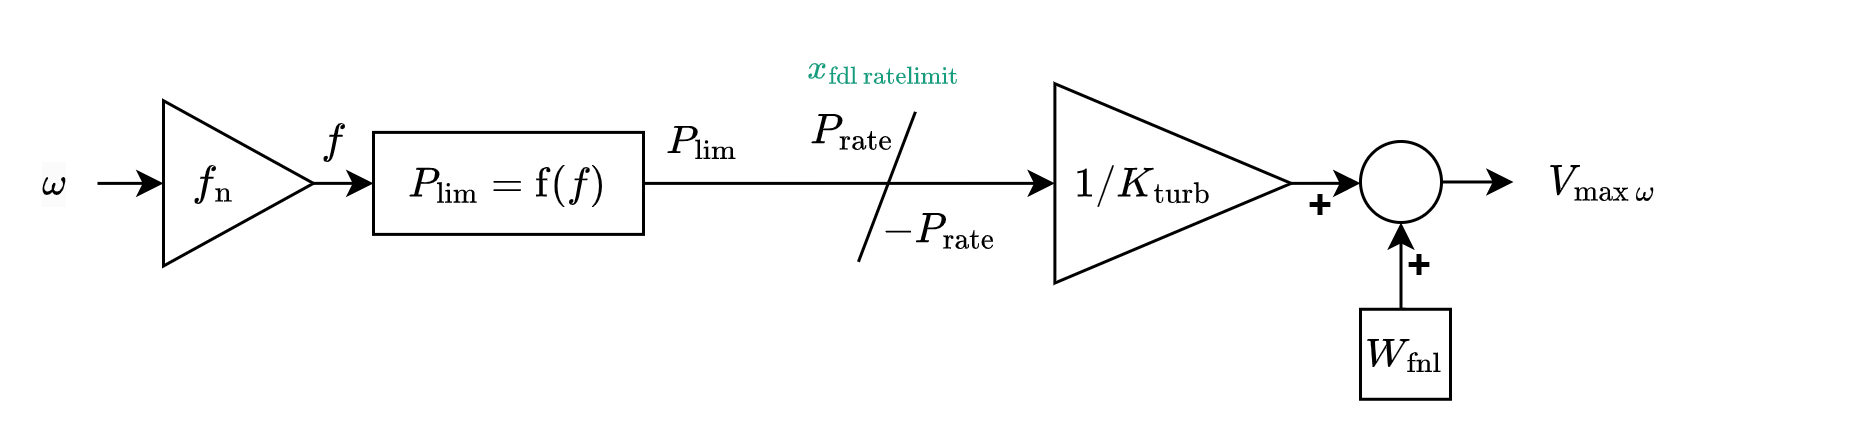
\includegraphics{drawings/GovCT2.frequencylimit.drawio.png}

}

\caption{\label{fig-frequencyDependentLimit}Frequency dependent valve
limit as described in {[}3{]}}

\end{figure}%

\subsection{Parameters}\label{parameters}

Per-unit power parameters are based on \(P_\mathrm{base}\), which is
normally the capability of the turbine in MW. Per-unit frequency or
acceleration parameters are based on the nominal frequency of the grid
(e.g.~50 Hz in Europe).

\begin{longtable}[]{@{}
  >{\raggedright\arraybackslash}p{(\columnwidth - 12\tabcolsep) * \real{0.0600}}
  >{\raggedright\arraybackslash}p{(\columnwidth - 12\tabcolsep) * \real{0.0600}}
  >{\raggedright\arraybackslash}p{(\columnwidth - 12\tabcolsep) * \real{0.0500}}
  >{\raggedright\arraybackslash}p{(\columnwidth - 12\tabcolsep) * \real{0.2000}}
  >{\raggedright\arraybackslash}p{(\columnwidth - 12\tabcolsep) * \real{0.1000}}
  >{\raggedright\arraybackslash}p{(\columnwidth - 12\tabcolsep) * \real{0.4400}}
  >{\raggedright\arraybackslash}p{(\columnwidth - 12\tabcolsep) * \real{0.0700}}@{}}
\caption{Parameters}\label{tbl-parameters}\tabularnewline
\toprule\noalign{}
\begin{minipage}[b]{\linewidth}\raggedright
name
\end{minipage} & \begin{minipage}[b]{\linewidth}\raggedright
type
\end{minipage} & \begin{minipage}[b]{\linewidth}\raggedright
unit
\end{minipage} & \begin{minipage}[b]{\linewidth}\raggedright
modelica name
\end{minipage} & \begin{minipage}[b]{\linewidth}\raggedright
IEC name
\end{minipage} & \begin{minipage}[b]{\linewidth}\raggedright
description
\end{minipage} & \begin{minipage}[b]{\linewidth}\raggedright
typical value
\end{minipage} \\
\midrule\noalign{}
\endfirsthead
\toprule\noalign{}
\begin{minipage}[b]{\linewidth}\raggedright
name
\end{minipage} & \begin{minipage}[b]{\linewidth}\raggedright
type
\end{minipage} & \begin{minipage}[b]{\linewidth}\raggedright
unit
\end{minipage} & \begin{minipage}[b]{\linewidth}\raggedright
modelica name
\end{minipage} & \begin{minipage}[b]{\linewidth}\raggedright
IEC name
\end{minipage} & \begin{minipage}[b]{\linewidth}\raggedright
description
\end{minipage} & \begin{minipage}[b]{\linewidth}\raggedright
typical value
\end{minipage} \\
\midrule\noalign{}
\endhead
\bottomrule\noalign{}
\endlastfoot
\(a_\mathrm{set}\) & float & pu/s & aSetPu & Aset & Acceleration limiter
setpoint & 10 \\
\(\Delta\omega_\mathrm{db}\) & float & pu & DeltaOmegaDbPu & db &
Frequency error deadband. Recommended to be =0 in most applications
{[}3{]} & 0 \\
\(\Delta\omega_\mathrm{max}\) & float & pu & DeltaOmegaMaxPu & Maxerr &
Maximum value for frequency error & 1 \\
\(\Delta\omega_\mathrm{min}\) & float & pu & DeltaOmegaMinPu & Minerr &
Minimum value for frequency error & -1 \\
\(\Delta t\) & float & s & DeltaT & \(\Delta t\) & Correction factor to
adapt the unit of \(K_\mathrm{a}\) from pu/s to pu & 1 \\
\(D_\mathrm{m}\) & float & pu & Dm & dm & Speed sensitivity coefficient,
see Section~\ref{sec-speedSensitivity} & 0 \\
\(f_\mathrm{lim\,1}\) & float & Hz & fLim1 & flim1 & Frequency threshold
1 & 59 \\
\(f_\mathrm{lim\,10}\) & float & Hz & fLim1 & flim10 & Frequency
threshold 10 & 0 \\
\(f_\mathrm{lim\,2}\) & float & Hz & fLim1 & flim2 & Frequency threshold
2 & 0 \\
\(f_\mathrm{lim\,3}\) & float & Hz & fLim1 & flim3 & Frequency threshold
3 & 0 \\
\(f_\mathrm{lim\,4}\) & float & Hz & fLim1 & flim4 & Frequency threshold
4 & 0 \\
\(f_\mathrm{lim\,5}\) & float & Hz & fLim1 & flim5 & Frequency threshold
5 & 0 \\
\(f_\mathrm{lim\,6}\) & float & Hz & fLim1 & flim6 & Frequency threshold
6 & 0 \\
\(f_\mathrm{lim\,7}\) & float & Hz & fLim1 & flim7 & Frequency threshold
7 & 0 \\
\(f_\mathrm{lim\,8}\) & float & Hz & fLim1 & flim8 & Frequency threshold
8 & 0 \\
\(f_\mathrm{lim\,9}\) & float & Hz & fLim1 & flim9 & Frequency threshold
9 & 0 \\
\(K_\mathrm{a}\) & float & pu & KA & Ka & Acceleration limiter gain &
10 \\
\(K_\mathrm{D\,gov}\) & float & pu & KDGov & Kdgov & Governor derivative
gain & 0 \\
\(K_\mathrm{I\,gov}\) & float & pu & KIGov & Kigov & Governor integral
gain & 0.45 \\
\(K_\mathrm{I\,load}\) & float & pu & KILoad & Kiload & Load limiter
integral gain & 1 \\
\(K_\mathrm{I\,MW}\) & float & pu & KIMw & Kimw & Supervisory load
controller integral gain & 0 \\
\(K_\mathrm{P\,gov}\) & float & pu & KPGov & Kpgov & Governor
proportional gain & 4 \\
\(K_\mathrm{P\,load}\) & float & pu & KPLoad & Kpload & Load limiter
proportional & 1 \\
\(K_\mathrm{turb}\) & float & pu & KTurb & Kturb & Turbine gain
(translates from fuel flow to power) & 1.9168 \\
\(P_\mathrm{base}\) & float & MW & PBaseMw & Mwbase & Base for power
values (\textgreater{} 0) & \\
\(P_\mathrm{ldref}\) & float & pu & PLdRefPu & Ldref & Load limiter
reference value & 1 \\
\(P_\mathrm{lim\,1}\) & float & pu & PLim1Pu & plim1 & Power limit 1 &
0.8325 \\
\(P_\mathrm{lim\,10}\) & float & pu & PLim10Pu & plim10 & Power limit 10
& 0 \\
\(P_\mathrm{lim\,2}\) & float & pu & PLim2Pu & plim2 & Power limit 2 &
0 \\
\(P_\mathrm{lim\,3}\) & float & pu & PLim3Pu & plim3 & Power limit 3 &
0 \\
\(P_\mathrm{lim\,4}\) & float & pu & PLim4Pu & plim4 & Power limit 4 &
0 \\
\(P_\mathrm{lim\,5}\) & float & pu & PLim5Pu & plim5 & Power limit 5 &
0 \\
\(P_\mathrm{lim\,6}\) & float & pu & PLim6Pu & plim6 & Power limit 6 &
0 \\
\(P_\mathrm{lim\,7}\) & float & pu & PLim7Pu & plim7 & Power limit 7 &
0 \\
\(P_\mathrm{lim\,8}\) & float & pu & PLim8Pu & plim8 & Power limit 8 &
0 \\
\(P_\mathrm{lim\,9}\) & float & pu & PLim9Pu & plim9 & Power Limit 9 &
0 \\
\(P_\mathrm{rate}\) & float & pu & PRatePu & prate & Ramp rate for
frequency-dependent power limit & 0.017 \\
\(R\) & float & pu & RDroop & R & Droop (frequency/power) & 0.05 \\
\(R_\mathrm{close}\) & float & pu/s & RClosePu & Rclose & Minimum rate
for valve closing & -99 \\
\(R_\mathrm{down}\) & float & pu & RDownPu & Rdown & temperature/load
limit path output decrease rate limit & -99 \\
\(R_\mathrm{open}\) & float & pu/s & ROpenPu & Ropen & Maximum rate for
valve closing & 99 \\
\(R_\mathrm{select}\) & int & - & RSelectInt & Rselect & governor
controller feedback mode switch & \\
\(R_\mathrm{up}\) & float & pu & RUpPu & Rup & temperature/load limit
path output increase rate limit & 99 \\
\(T_\mathrm{a}\) & float & s & tA & Ta & Acceleration limiter time
constant & 1 \\
\(T_\mathrm{act}\) & float & s & tActuator & Tact & actuator (valve)
reaction time constant & 0.4 \\
\(T_\mathrm{b}\) & float & s & tB & Tb & Turbine lag time constant &
0.1 \\
\(T_\mathrm{c}\) & float & s & tC & Tc & Turbine lead time constant &
0 \\
\(T_\mathrm{dgov}\) & float & s & tDGov & Tdgov & Governor controller
derivative time constant & 1 \\
\(T_\mathrm{D\,ratelim}\) & float & s & tDRatelim & - & Ramp rate limter
derivative time constant in s & 0.001 \\
\(T_\mathrm{eng}\) & float & s & tEngine & Teng & Transport time delay
for diesel engine & 0 \\
\(T_\mathrm{f\,load}\) & float & s & tFLoad & Tfload & Load limiter time
constant & 3 \\
\(T_\mathrm{last\,value}\) & float & s & tLastValue & - & Time constant
of very fast first order block to prevent algebraic loop & 1e-9 \\
\(T_\mathrm{p\,elec}\) & float & s & tPElec & Tpelec & Electrical power
measurement time constant & 2.5 \\
\(T_\mathrm{sa}\) & float & s & tSA & Tsa & lead time constant of
temperature detection & 0 \\
\(T_\mathrm{sb}\) & float & s & tSB & Tsb & lag time constant of
temperature detection & 50 \\
\(V_\mathrm{max}\) & float & pu & ValveMaxPu & Vmax & Maximum valve
position limit & 1 \\
\(V_\mathrm{min}\) & float & pu & ValveMinPu & Vmin & Minimum valve
position limit & 0.175 \\
\(W_\mathrm{fnl}\) & float & pu & WFnlPu & Wfnl & fuel flow with no load
& 0.187 \\
\(W_\mathrm{fspd}\) & bool & - & WFSpdBool & Wfspd & Switch for fuel
source characteristic & false \\
\end{longtable}

\subsection{Variables}\label{variables}

\subsubsection{Inputs}\label{inputs}

\begin{longtable}[]{@{}
  >{\raggedright\arraybackslash}p{(\columnwidth - 10\tabcolsep) * \real{0.0600}}
  >{\raggedright\arraybackslash}p{(\columnwidth - 10\tabcolsep) * \real{0.0600}}
  >{\raggedright\arraybackslash}p{(\columnwidth - 10\tabcolsep) * \real{0.0500}}
  >{\raggedright\arraybackslash}p{(\columnwidth - 10\tabcolsep) * \real{0.2000}}
  >{\raggedright\arraybackslash}p{(\columnwidth - 10\tabcolsep) * \real{0.1000}}
  >{\raggedright\arraybackslash}p{(\columnwidth - 10\tabcolsep) * \real{0.4400}}@{}}
\caption{Inputs}\label{tbl-inputs}\tabularnewline
\toprule\noalign{}
\begin{minipage}[b]{\linewidth}\raggedright
name
\end{minipage} & \begin{minipage}[b]{\linewidth}\raggedright
type
\end{minipage} & \begin{minipage}[b]{\linewidth}\raggedright
unit
\end{minipage} & \begin{minipage}[b]{\linewidth}\raggedright
modelica name
\end{minipage} & \begin{minipage}[b]{\linewidth}\raggedright
IEC name
\end{minipage} & \begin{minipage}[b]{\linewidth}\raggedright
description
\end{minipage} \\
\midrule\noalign{}
\endfirsthead
\toprule\noalign{}
\begin{minipage}[b]{\linewidth}\raggedright
name
\end{minipage} & \begin{minipage}[b]{\linewidth}\raggedright
type
\end{minipage} & \begin{minipage}[b]{\linewidth}\raggedright
unit
\end{minipage} & \begin{minipage}[b]{\linewidth}\raggedright
modelica name
\end{minipage} & \begin{minipage}[b]{\linewidth}\raggedright
IEC name
\end{minipage} & \begin{minipage}[b]{\linewidth}\raggedright
description
\end{minipage} \\
\midrule\noalign{}
\endhead
\bottomrule\noalign{}
\endlastfoot
\(\omega\) & float & pu & omegaPu & \(\omega\) & rotor speed \\
\(P_\mathrm{ref}\) & float & pu & PRefPu & Pref & load setpoint \\
\(P_\mathrm{MWSet}\) & float & pu & PMwSetPu & Pmwset & Supervisory
power controller setpoint (automatic generation control) \\
\(P_\mathrm{e}\) & float & pu & PGenPu & Pe & measured electric power
generation \\
\end{longtable}

\subsection{Outputs}\label{outputs}

\begin{longtable}[]{@{}
  >{\raggedright\arraybackslash}p{(\columnwidth - 10\tabcolsep) * \real{0.0600}}
  >{\raggedright\arraybackslash}p{(\columnwidth - 10\tabcolsep) * \real{0.0600}}
  >{\raggedright\arraybackslash}p{(\columnwidth - 10\tabcolsep) * \real{0.0500}}
  >{\raggedright\arraybackslash}p{(\columnwidth - 10\tabcolsep) * \real{0.2000}}
  >{\raggedright\arraybackslash}p{(\columnwidth - 10\tabcolsep) * \real{0.1000}}
  >{\raggedright\arraybackslash}p{(\columnwidth - 10\tabcolsep) * \real{0.4400}}@{}}
\caption{Outputs}\label{tbl-outputs}\tabularnewline
\toprule\noalign{}
\begin{minipage}[b]{\linewidth}\raggedright
name
\end{minipage} & \begin{minipage}[b]{\linewidth}\raggedright
type
\end{minipage} & \begin{minipage}[b]{\linewidth}\raggedright
unit
\end{minipage} & \begin{minipage}[b]{\linewidth}\raggedright
modelica name
\end{minipage} & \begin{minipage}[b]{\linewidth}\raggedright
IEC name
\end{minipage} & \begin{minipage}[b]{\linewidth}\raggedright
description
\end{minipage} \\
\midrule\noalign{}
\endfirsthead
\toprule\noalign{}
\begin{minipage}[b]{\linewidth}\raggedright
name
\end{minipage} & \begin{minipage}[b]{\linewidth}\raggedright
type
\end{minipage} & \begin{minipage}[b]{\linewidth}\raggedright
unit
\end{minipage} & \begin{minipage}[b]{\linewidth}\raggedright
modelica name
\end{minipage} & \begin{minipage}[b]{\linewidth}\raggedright
IEC name
\end{minipage} & \begin{minipage}[b]{\linewidth}\raggedright
description
\end{minipage} \\
\midrule\noalign{}
\endhead
\bottomrule\noalign{}
\endlastfoot
\(P_\mathrm{m}\) & float & pu & PmPu & Pm & mechanical power \\
\end{longtable}

\subsection{Equations \& algorithm ~}\label{equations-algorithm}

--

\subsection{Initial equations / boundary
conditions}\label{initial-equations-boundary-conditions}

The initial values for the system's states are calculated from the
initial mechanical power \(P_\mathrm{m\,0}\) and rotation speed
\(\omega_\mathrm{0}\).

\subsubsection{Helper variables}\label{helper-variables}

The following \emph{helper variables} are defined to avoid repetition in
the definitions of initial states below. They are the initial values of
signals at certain points in Figure~\ref{fig-modelSchema}.

\begin{equation}\phantomsection\label{eq-initPmnoloss}{
P_\mathrm{m\,noloss\,0} = 
\begin{cases}
    P_\mathrm{m\,0} + \omega_\mathrm{0} \cdot D_\mathrm{m},& \text{if } D_\mathrm{m}> 0\\
    P_\mathrm{m\,0},              & \text{otherwise}
\end{cases}
}\end{equation}

\begin{equation}\phantomsection\label{eq-initCfe}{
C_\mathrm{fe\,0} = 
\begin{cases}
    W_\mathrm{fnl} + P_\mathrm{m\,noloss\,0} / K_\mathrm{turb},& \text{if } K_\mathrm{turb}>0\\
    W_\mathrm{fnl},              & \text{otherwise}
\end{cases}
}\end{equation}

\begin{equation}\phantomsection\label{eq-initValve}{
V_\mathrm{0} = 
\begin{cases}
    C_\mathrm{fe\,0} / \omega_\mathrm{0},& \text{if } W_\mathrm{fspd}\\
    C_\mathrm{fe\,0},              & \text{otherwise}
\end{cases}
}\end{equation}

\begin{equation}\phantomsection\label{eq-initTex}{
\vartheta_\mathrm{ex\,0} = 
\begin{cases}
    C_\mathrm{fe\,0} \cdot \omega_\mathrm{0}^{D_\mathrm{m}},& \text{if } D_\mathrm{m}<0\\
    1,              & \text{otherwise}
\end{cases}
}\end{equation}

\begin{equation}\phantomsection\label{eq-initFsrt}{
F_\mathrm{srt\,0} = (P_\mathrm{ldref}/K_\mathrm{turb} + W_\mathrm{fnl} - \vartheta_\mathrm{ex\,0}) \cdot K_\mathrm{P\,load} + x_\mathrm{I\,load}
}\end{equation}

\subsubsection{Initial states}\label{initial-states}

\begin{equation}\phantomsection\label{eq-initXiload}{
x_\mathrm{I\,load\,0} = 1
}\end{equation}

\begin{equation}\phantomsection\label{eq-initXTurbine}{
x_\mathrm{turb\,0} = P_\mathrm{m\,noloss\,0}
}\end{equation}

\begin{equation}\phantomsection\label{eq-initXValve}{
x_\mathrm{valve\,0} = V_\mathrm{0}
}\end{equation}

\begin{equation}\phantomsection\label{eq-initXFdl}{
x_\mathrm{fdl\,ratelimit\,0} = K_\mathrm{turb}(V_\mathrm{max}-W_\mathrm{fnl})
}\end{equation}

\begin{equation}\phantomsection\label{eq-initXIGov}{
x_\mathrm{I\,gov\,0} = V_\mathrm{0}
}\end{equation}

\begin{equation}\phantomsection\label{eq-initXMeasPe}{
x_\mathrm{meas\,Pe\,0} = P_\mathrm{m\,0}
}\end{equation}

\begin{equation}\phantomsection\label{eq-initFsrt}{
x_\mathrm{fsrt\,ratelim\,0} = F_\mathrm{srt\,0}
}\end{equation}

\begin{equation}\phantomsection\label{eq-Texm}{
x_\mathrm{meas\,\vartheta\,ex\,0} = \vartheta_\mathrm{ex\,0}
}\end{equation}

\begin{equation}\phantomsection\label{eq-initTex}{
x_\mathrm{\vartheta\,ex\,0} = \vartheta_\mathrm{ex\,0}
}\end{equation}

\begin{equation}\phantomsection\label{eq-initXIMw}{
x_\mathrm{I\,MW} = 0
}\end{equation}

\begin{equation}\phantomsection\label{eq-initLastValue}{
x_\mathrm{last\,value\,0} = V_\mathrm{0}
}\end{equation}

\begin{equation}\phantomsection\label{eq-initFsra}{
x_\mathrm{fsra\,0} = 0
}\end{equation}

\subsubsection{Initial power reference}\label{initial-power-reference}

\begin{equation}\phantomsection\label{eq-initPRef}{
P_\mathrm{ref\,0} = 
\begin{cases}
    0,                         & \text{if } R_\mathrm{select}=0\\
    R \cdot P_\mathrm{m\,0},   & \text{if } R_\mathrm{select}=1\\
    R \cdot V_\mathrm{0},      & \text{otherwise}
\end{cases}
}\end{equation}

\section{Assumptions in modelica implementation (Open source
implementations)}\label{assumptions-in-modelica-implementation-open-source-implementations}

\subsection{Base values}\label{base-values}

\begin{itemize}
\tightlist
\item
  PGenPu has base SystemBase.SnRef

  \begin{itemize}
  \tightlist
  \item
    A change of base has been added just after the input connector
  \end{itemize}
\item
  PRefPu has base PNomTurb/RDroop
\item
  Output PmPu has base PNomTurb
\end{itemize}

\subsection{Integrator anti-windup and integrator
limits}\label{integrator-anti-windup-and-integrator-limits}

\subsubsection{Limits}\label{sec-assumptionLimits}

In {[}3{]} (page 45) it is stated that generally \emph{``limited
integrators are of the non-windup type''}. A concrete implementation is
not specified. On p.~244 IEEE 421.5-2005 anti windup is referenced, but
related to an AVR model. Since in {[}3{]} (Fig. 48) there is an
explicitly limited integrator (\texttt{Kimw}), it was assumed that the
integrators \texttt{Kigov} and \texttt{Kiload} are not \emph{limited} in
that sense, they are merely integrators with limits after them. Hence,
they do not have a limit.

\subsubsection{Anti-windup}\label{anti-windup}

In {[}3{]} (Fig. 47) it is shown for the GovCT1 model that the
\(K_\mathrm{I\,gov}\) and \(K_\mathrm{I\,load}\) integrators have a
so-colled \emph{tracking logic}, i.e.~anti-windup logic, implemented.

For GovCT2, there are two statements:

\begin{enumerate}
\def\labelenumi{\arabic{enumi})}
\item
  In {[}3{]} (p.~139) it is stated that \textgreater{} The Kpgov/Kigov
  and Kpload/Kiload controllers include tracking logic to ensure smooth
  transfer between active controllers. This logic is not shown on the
  GovCT2 diagram.
\item
  Just above that, the following is written: \textgreater{} Aside from
  the frequency-dependent limit, GovCT2 is identical to GovCT1, except
  that the temperature fuel command fsrt does not track fsr when it is
  not in control. Instead, it stays at its upper limit (1).
\end{enumerate}

Statement 2. contradicts in two ways:

\begin{itemize}
\tightlist
\item
  it says that there is no tracking logic for the \(K_\mathrm{I\,load}\)
  integrator, while statement 1) says the opposite.
\item
  it says that there is an upper limit on the \(K_\mathrm{I\,load}\)
  controller, which contradicts Section~\ref{sec-assumptionLimits}.
\end{itemize}

\subsubsection{Resulting assumptions}\label{resulting-assumptions}

The validation reference model in DIgSILENT PowerFactory does not
include the tracking logic. Because of this and the contradicting
informaton in the standard:

\begin{itemize}
\tightlist
\item
  No tracking logic has been implemented
\item
  Integrator limits are only implemented if explicitly shown in {[}3{]}
  (Fig. 48)
\end{itemize}

\subsection{Ramp rate limiters}\label{ramp-rate-limiters}

As ramp rate limiter, the Modelica library block
\texttt{Modelica.Blocks.Nonlinear.SlewRateLimiter} is used.

\begin{quote}
The SlewRateLimiter block limits the slew rate of its input signal in
the range of {[}Falling, Rising{]}. To ensure this for arbitrary inputs
and in order to produce a differential output, the input is numerically
differentiated with derivative time constant Td. Smaller time constant
Td means nearer ideal derivative. Note: The user has to choose the
derivative time constant according to the nature of the input signal.
\end{quote}

\emph{Documentation of the Modelica block}

\begin{itemize}
\tightlist
\item
  The default value of \(T_\mathrm{D\,ratelim}=1 \mathrm{ms}\) is used.
\item
  The same value is used for each ramp rate limiter block.
\end{itemize}

\subsection{\texorpdfstring{Input signals \(\omega\) and
\(P_\mathrm{ref}\)}{Input signals \textbackslash omega and P\_\textbackslash mathrm\{ref\}}}\label{input-signals-omega-and-p_mathrmref}

\subsubsection{\texorpdfstring{Power setpoint
\(P_\mathrm{ref}\)}{Power setpoint P\_\textbackslash mathrm\{ref\}}}\label{power-setpoint-p_mathrmref}

Since the power feedback gets passed through the droop \(R\), so for the
power difference to make sense, the reference power needs to be
multiplied by \(R\) as well. This has historical reasons, see {[}1{]}
section 2.3.3.5 (before digital times it used to be a mechanical lever
that is moved, it did not matter what the lever positions meant).

\begin{itemize}
\tightlist
\item
  \textbf{assumption:} In this implementation the reference power input
  needs to be multiplied by \(R\) before entering the governor model.
\end{itemize}

The same is done in \emph{DIgSILENT PowerFactory} GovCT2 at
initialization: \texttt{inc(Pref)\ =\ R*Pfdbck\ +\ w}. ()

\subsubsection{\texorpdfstring{Rotor speed
\(\omega\)}{Rotor speed \textbackslash omega}}\label{rotor-speed-omega}

\begin{itemize}
\tightlist
\item
  In \emph{DIgSILENT PowerFactory}, different implementations for the
  speed signal are used. For example,

  \begin{itemize}
  \tightlist
  \item
    In the PSS/E compatible GGOV1 model, the reference speed is
    explicitly subtracted from the measured speed to calculate
    \texttt{dw}, which is then subtracted at the control error summation
    point. Here, the reference power input is initialized to
    \texttt{inc(Pref)\ =\ R*Pfdbck+dw}.
  \item
    In the GovCT2 model, the speed \texttt{w} is directly subtracted at
    the control error summation point. Here, the reference power input
    is initialized to \texttt{inc(Pref)\ =\ R*Pfdbck+w}.
  \item
    So in both cases the initial speed value that is subtracted from the
    control error summation point is -- implicitly! -- being added to
    that summation point through the \texttt{Pref} input. The effect is
    that in both cases \(\Delta \omega\) is subtracted at the summation
    point.
  \end{itemize}
\item
  In the CGMES standard {[}3{]}, two points remain unclear:

  \begin{itemize}
  \tightlist
  \item
    The input \(\omega\) is passed into the summation point while it
    should be \(\Delta \omega\). In {[}4{]}, \(\omega - 1\) is used as
    input, which supports this claim.
  \item
    The input \emph{speed} on the bottom right in {[}3{]} (Fig. 48)
    should be the same as \(\omega\), which is also backed by {[}4{]}.
  \end{itemize}
\item
  \textbf{assumption:} In this model, this subtraction is being done
  explicitly by calculating \(\Delta \omega = \omega - 1\) (see
  Figure~\ref{fig-modelSchema}) and \textbf{not} adding anything speed
  related to the power reference input.
\end{itemize}

\subsection{Frequency-dependent limit}\label{frequency-dependent-limit}

The mapping between frequency and maximum valve position is implemented
via a lookup table. The table consists of 10 pairs of values. Successive
values need to decrease in frequency and max. power. If e.g.~only 5
pairs shall be used instead of all 10, only define pairs 1 to 5 and set
all following pairs with fLim=0 and PLim = PLim5, resuling in a straight
line in the lookup table. \textbf{This is implemented slightly different
compared to {[}3{]} (p.~139).}

\subsection{Governor output feedback
delay}\label{governor-output-feedback-delay}

To prevent an algebraic loop when using the governor output feedback, a
first-order lag block with time constant \(T_\mathrm{last\,value}\) has
been added to the governor output feedback loop. The use of a unit delay
block (1/z) has been found impractical.

\section{Table of references}\label{table-of-references}

\phantomsection\label{refs}
\begin{CSLReferences}{0}{0}
\bibitem[\citeproctext]{ref-machowski2020}
\CSLLeftMargin{{[}1{]} }%
\CSLRightInline{J. Machowski, Z. Lubosny, J. W. Bialek, and J. R. Bumby,
\emph{Power {System Dynamics}: {Stability} and {Control}, 3rd
{Edition}}. Wiley, 2020. Accessed: Nov. 22, 2022. {[}Online{]}.
Available:
\url{https://www.wiley.com/en-us/Power+System+Dynamics\%3A+Stability+and+Control\%2C+3rd+Edition-p-9781119526360}}

\bibitem[\citeproctext]{ref-alliander2024}
\CSLLeftMargin{{[}2{]} }%
\CSLRightInline{alliander, {``Alliander-opensource.''} {[}Online{]}.
Available:
\url{https://alliander-opensource.github.io/cgmes-profiles/Dynamics/GovCT2/}}

\bibitem[\citeproctext]{ref-iec61970-3022023}
\CSLLeftMargin{{[}3{]} }%
\CSLRightInline{IEC61970-302, {``{DIN EN IEC} 61970-302 --
{Schnittstelle} für {Anwendungsprogramme} für {Energiemanagementsysteme}
({EMS}­{API}) {Teil}~302: {Allgemeines Informationsmodell}~({CIM})
{Dynamik}.''} Jun. 2023.}

\bibitem[\citeproctext]{ref-neplan2015}
\CSLLeftMargin{{[}4{]} }%
\CSLRightInline{Neplan, {``{TURBINE-GOVERNOR MODELS} -- {Standard
Dynamic Turbine-Governor Systems} in {NEPLAN Power System Analysis
Tool}.''} 2015. Available: \href{https://www.neplan.ch}{www.neplan.ch}}

\end{CSLReferences}




\end{document}
